\chapter{Upgrade of the Pixel Tracker}\label{chapt:pixel}

The CMS detector as described in chapter \ref{chap:exp_setup} was performing during the time period 
between 2010 and 2012. It provided a center-of-mass energy up to 8 TeV and the bunch spacing was 50 ns. 
However, the LHC program was planned for at least a decade longer and the plan includes several improvements.

After the shutdown for two years, from the end of 2012 until the beginning of 2015, the LHC 
center-of-mass energy was increased up to 13 TeV and will be further increased to the designed value
of 14 TeV. The next long shutdown is planned in 2018. Until that time it is planned that the peak
luminosity will reach $10^{34} \text{cm}^{-2} \text{s}^{-1}$ (comparing to the $7 \cdot 10^{33} \text{cm}^{-2}\text{s}^{-1}$
reached in 2012). The total integrated luminosity which is planned to achieve prior the second long shutdown
is 100 fb$^{-1}$ \cite{CMS:2012sda}. This LHC phase is called \textit{Phase 0}.

The plan after the second long shutdown (2018) is to increase the brightness of the bunches
in the accelerators. This is planned to be done with improving the injectors. In the period 
after a second long shut down and until 2022 (so-called \textit{Phase 1}) the LHC will reach
a peak luminosity of $2-3 \cdot 10^{34} \text{cm}^{-2} \text{s}^{-1}$ and deliver about 
300 fb$^{-1}$ of data \cite{Rocca:2014soa}. 

The third long shutdown in 2022-2023 will be used for the improvements of the LHC accelerating system by
exchanging the aged parts by the new and improved ones (focusing magnets, cryogenics system, etc.).
After these improvements, the LHC is expected to reach a peak luminosity of $2-3 \cdot 10^{34} \text{cm}^{-2} \text{s}^{-1}$.
The period of LHC operation after the third long shut down is called \textit{Phase 2} \cite{Rocca:2014soa}.

It is natural that the changes of the accelerator systems have to be reflected also in the detector construction.
If the collisions with higher energies and frequencies are provided by the accelerator machine, the detector might
be overloaded with information and some of its parts might be damaged by the higher radiation. That is why 
the CMS is also being upgraded simultaneously with the LHC.

The silicon pixel tracker (see the description in sec. \ref{sec:tracker}) is the innermost part of the CMS 
detector mounted around the beam pipe and being the closest detector to the collision point. That means that
it receives the highest irradiation dose and operates in a very dense particle environment. After the upgrade 
in 2015 the conditions for the pixel tracker will get even more severe. That is why it has to be significantly 
upgraded to perform with the sufficient precision. 

This chapter describes the studies performed in frames of the fourth layer barrel pixel detector upgrade for the
LHC Phase 1. It is mainly concentrated on the barrel pixel tracker, and specifically on the tests for the
planned fourth layer of the latter.

\section{Plan For the Upgrade of the Barrel Pixel Tracker}

This section will give a brief overview of the plan for the whole CMS silicon pixel upgrade in frames of so-called
Phase I upgrade. The purpose of this upgrade is to remake and update the present silicon pixel tracker to make it 
suitable for the high luminosity and energy runs which will start after the year 2016. The replacement of the silicon
pixel tracker is planned for the technical stop in 2016/2017. 

The main goal for the updated pixel detector is that it should function at higher luminosities with the same or even
better performance as the current pixel tracker on the lower luminosities \cite{CMS:2012sda}. For these needs new read-out chips
(ROCs) have to be designed such that the data losses are minimized. In addition, the readout system as well as all
the other detector components have to be radiation hard, as the expected doses which the detector has to meet (especially
the first layer, which is the closest to the beam pipe) are much increased.

It was also decided to increase the number of barrel layers of the pixel detector from 3 to 4 (see Fig. \ref{fig:tracker_4}).
They were designed as four concentric cylinders with a length of 548.8 mm and radii between 30 mm and 160 mm.
This improves the track identification, which is crucial in the environment with a twice higher pile-up, expected for the 
LHC run after 2017. In addition the innermost layer of the detector is moved closer to the collision point (by 10 mm), while
the layers 2 and 3 are almost unchanged in the position. The beam pipe
will also be made smaller to allow the closer approach to the interactions.

Each layer will constructed of various number of 22 mm wide facets, in total consisting of 1184 rectangular pixel modules. Each module
consists of 16 pixel chips. The total number of pixels will be increased from roughly 48 M to 79 M.

\begin{figure}[t]
 \centering
 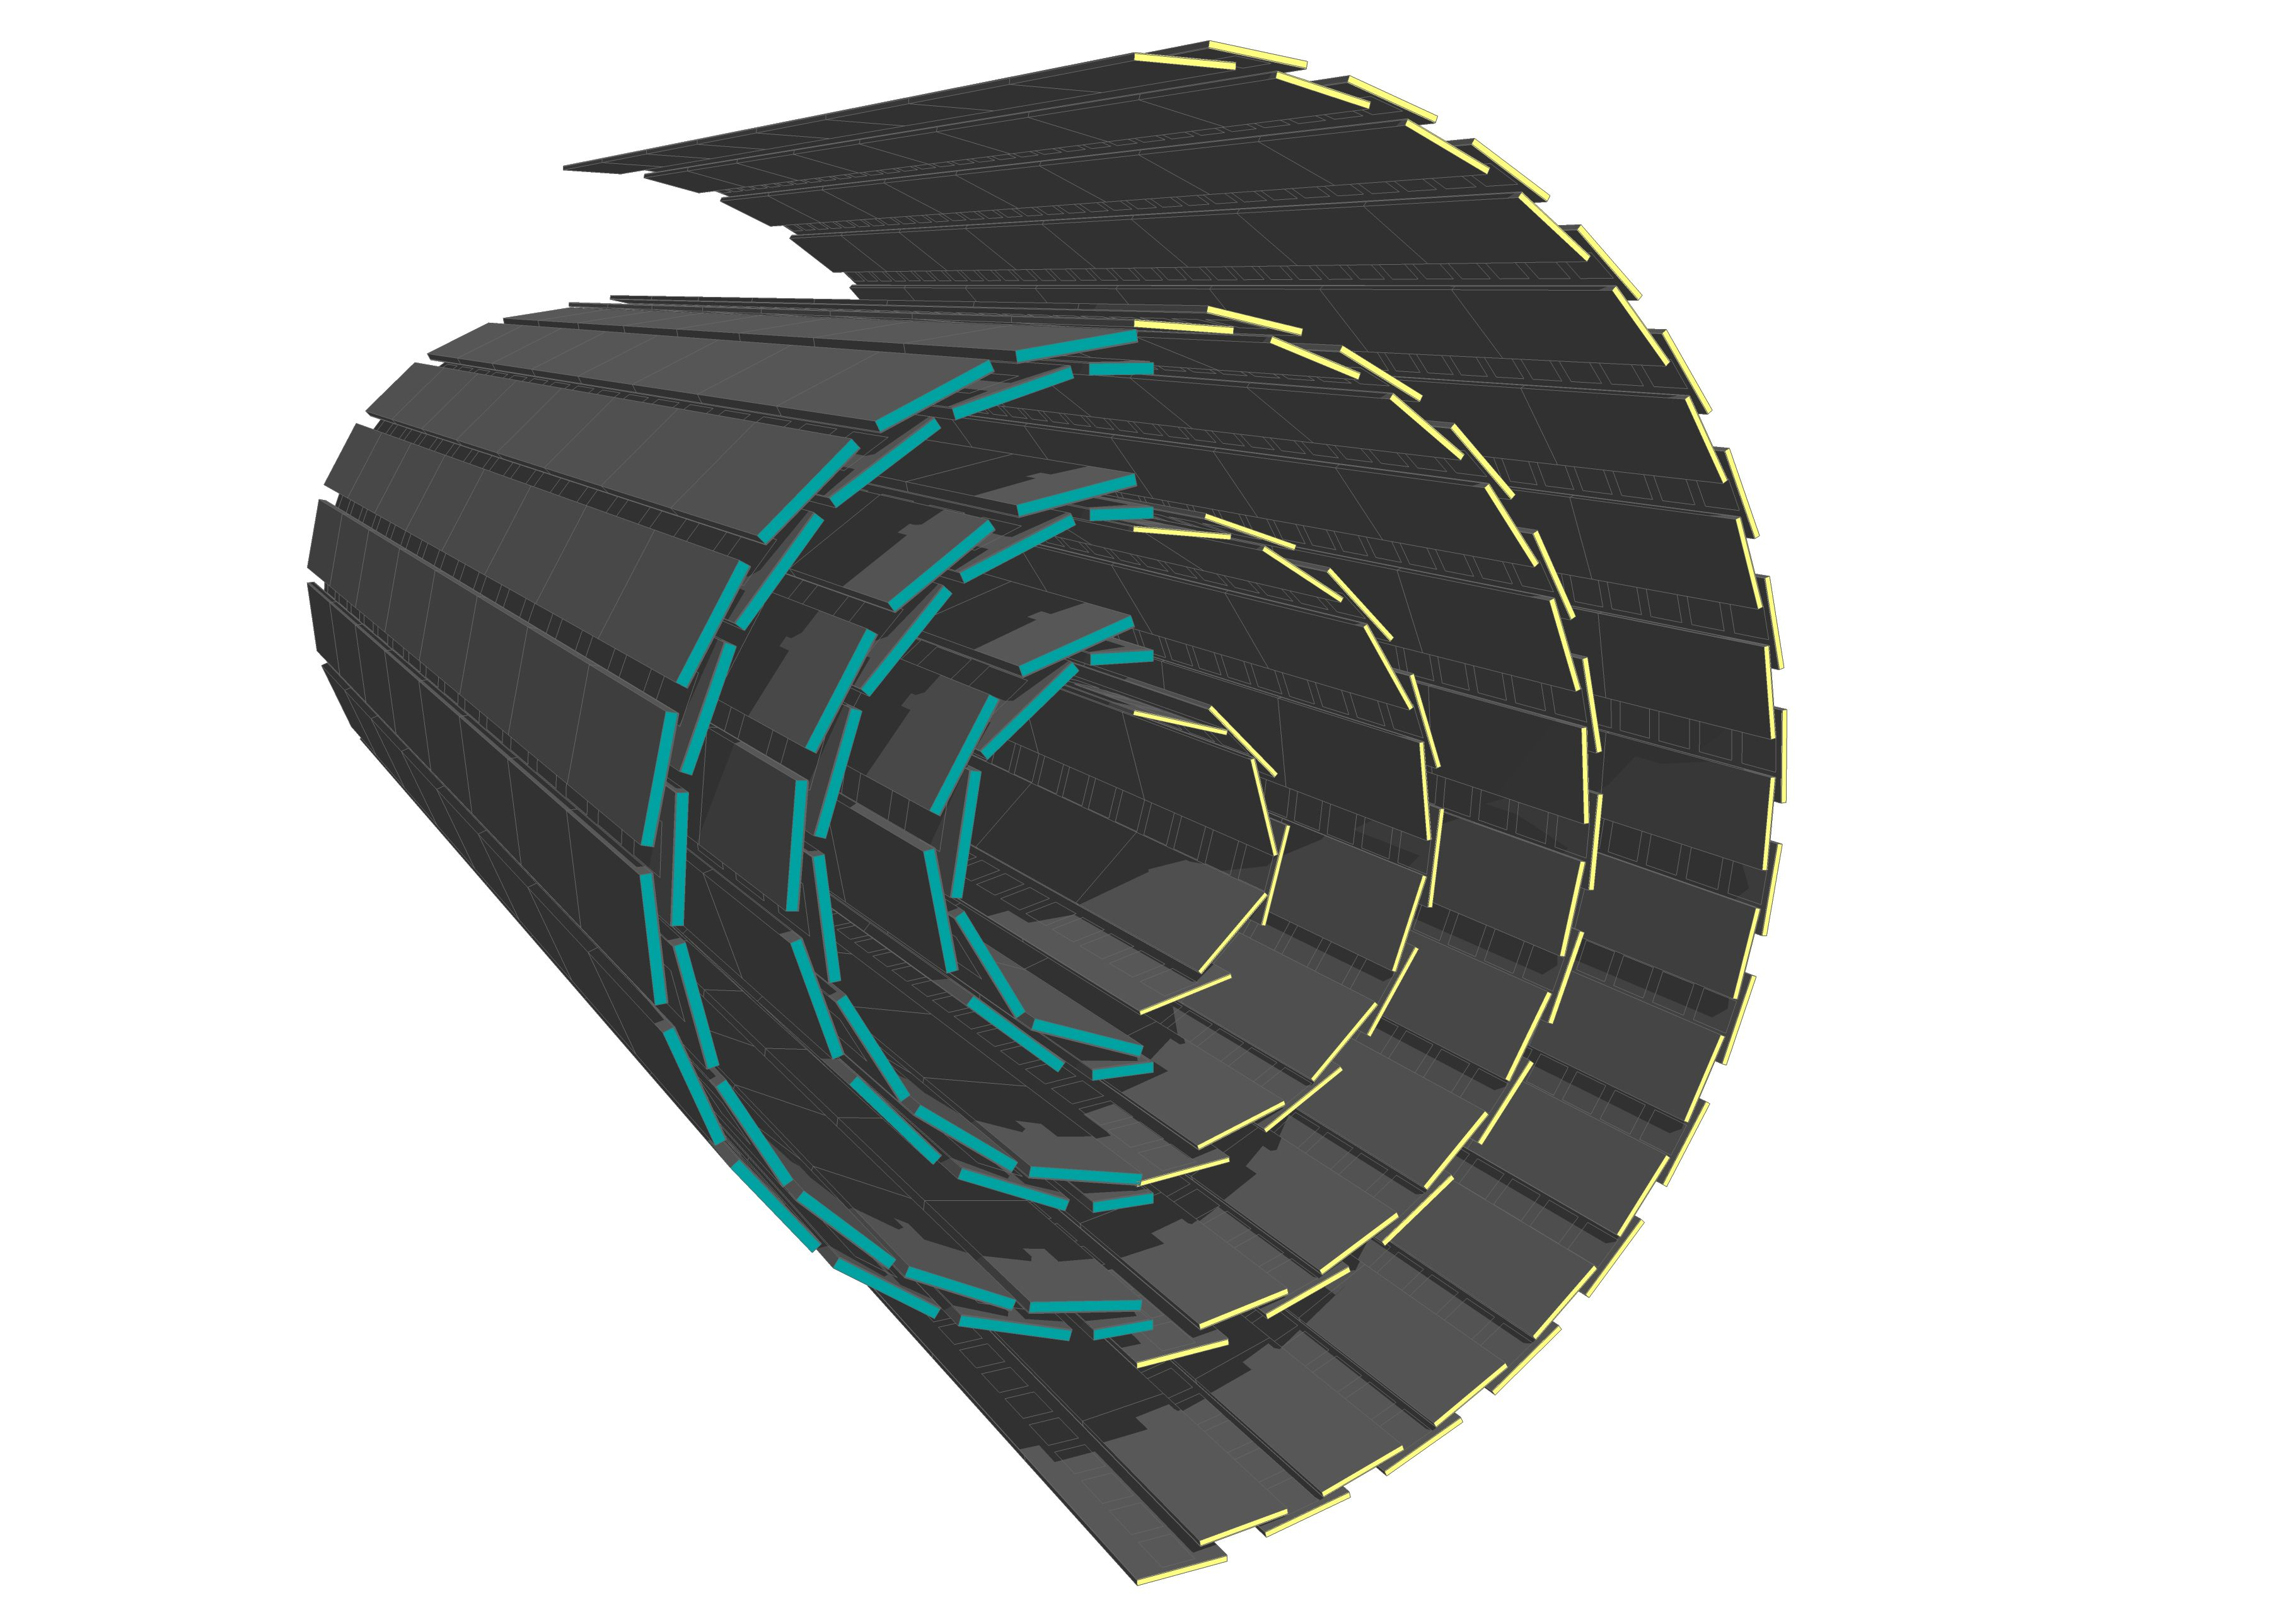
\includegraphics[width=1.0\textwidth]{021_pixel_upgrade/plots/pixel_phase1_4_layers.png}
 \caption{The model of the barrel pixel tracker before (on the left) and after the Phase 1 upgrade (on the right). Figure taken from
 \cite{CMS:2012sda}.}
 \label{fig:tracker_4}
\end{figure}

The addition of the fourth layer increases the amount of material which the particles have to go through. This is not
the desired feature for the innermost detectors. So the volume of the material, which the detector is made of, has to be decreased. 
First of all, the readout system itself is planned to be thinner (it is easy to see in the Fig. \ref{fig:tracker_4},
where the new pixel barrels are thinner). Secondly, the electronic boards will be moved out of the detector volume. 
Additionally, a new $CO_{2}$ cooling system \cite{CMS:2012sda} with a light-weight mechanical support will save material budget.

The improvements planned will lead to higher efficiencies, lower fake track rates (see sec. \ref{ssec:trkReco}), lower read-out dead time,
and extended lifetime of the detector. This results in a better identification of the particles for offline analysis and HLT.

The planned upgraded detector performance was simulated. It was compared to the performance of the non-upgraded tracker. This comparison
is shown in Fig. \ref{fig:sim_perform}. These simulations were performed on the simulated $t\bar{t}$ samples. The studies show overall higher 
efficiencies and lower fake rates for the upgrade detector for the higher puleup scenarios.

\begin{figure}[p]
 \centering
 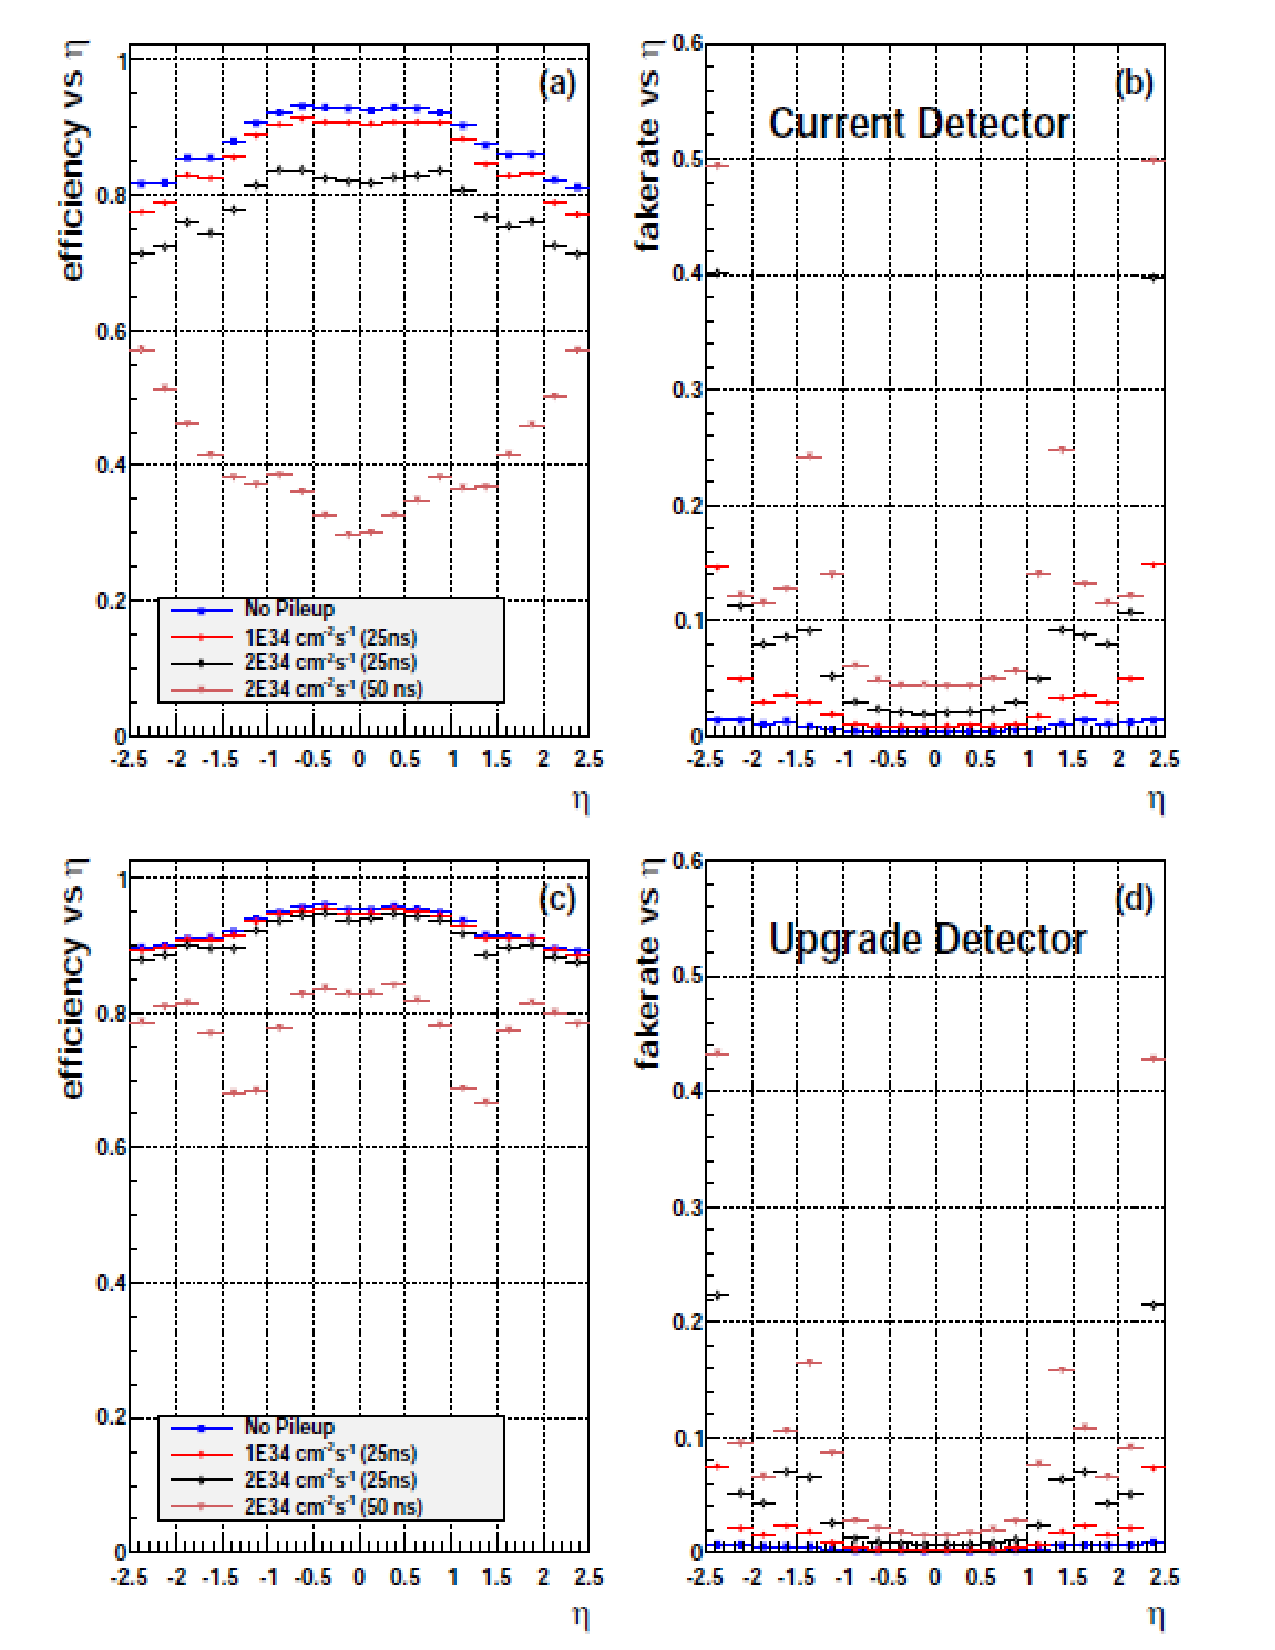
\includegraphics[width=0.8\textwidth]{021_pixel_upgrade/plots/sim_perform.pdf}
 \caption{Tracking efficiency (a,c) and fake rate (b,d) for the simulated $t\bar{t}$ sample as a function of track
          pseudorapidity $\eta$, for the current detector (a,b) and the upgrade pixel detector (c,d). Results are shown for
          zero pileup (blue squares), an average pileup of 25 (red dots), an average pileup of 50 (black
          diamonds), and an average pileup of 100 (brown triangles). The ROC data losses were simulated
          as expected at each given luminosity. The plot is taken from \cite{CMS:2012sda}.}
 \label{fig:sim_perform}
\end{figure}


\section{Studies of Irradiated Prototype Modules}

The expected performance of the barrel pixel tracker was confirmed in the simulated experiments. However, it is also crucial to test 
the performance of the device under real conditions. 

Prototype single chips were produced for the needs of such tests. These are chips of the design which was meant for the production
of the real detector facility, but supplemented with a separate readout system and board to enable an independent operation of such
a chip. 

In this work tests of the prototype chips for the fourth layer barrel pixel (BPIX) detector were performed. The layout of the prototype chip is shown 
in Fig. \ref{fig:prototype}. The chip is a 1/16 part of the modules from which the pixel detector will consist. 
One prototype chip contains 80 rows and 52 columns of pixels, each of the size $100\times150$ $\mu$m$^{2}$.
These pixels collect electrons from oxygenated high-resistivity $n$-type silicon sensors of 285 $\mu$m thickness with n+ implants. 

\begin{figure}[t]
 \centering
 \begin{subfigure}
  \centering
  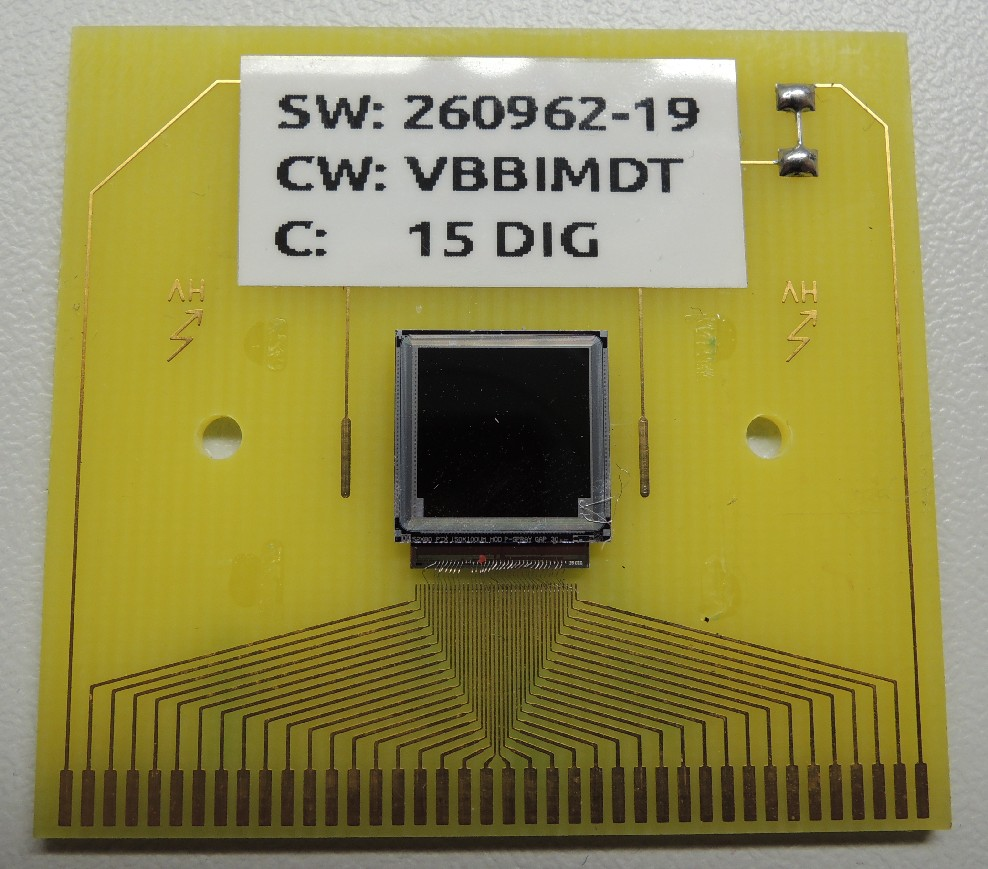
\includegraphics[width=0.4\textwidth]{021_pixel_upgrade/plots/prototype_chip_photo.png}
 \end{subfigure}
 \begin{subfigure}
  \centering
  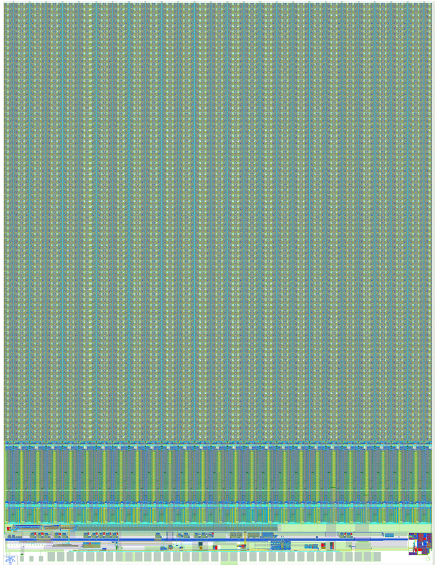
\includegraphics[width=0.4\textwidth]{021_pixel_upgrade/plots/prototype_chip.png}
 \end{subfigure}
 \caption{The photo of the prototype silicon pixel chip for the Phase I upgrade of the CMS BPIX, layer 4, mounted to the readout panel (on the left)
 and a magnified readout chip layout print (on the right).}
 \label{fig:prototype}
\end{figure}

Each pixel is bump-bonded to the ROC of the same height and width. The ROCs are fabricated in 250 nm CMOS (Complementary Metal-Oxide-Semiconductor)
employing the radiation hard design rules.
For the upgrade, the data buffer is increased to be able to work with higher occupancy connected with the higher data flow from the more frequent 
and dense LHC collisions. Furthermore the measured charges are digitalized and transmitted at 160 MHz. The effect of the internal cross talk is reduced
by design optimization and use of the 6 metal layers for the circuit, which allowed to operate at lower thresholds.

One of the important tests was to examine the chips with new design with respect to their radiation hardness. As discussed before the
pixel detector will receive the maximum dose of the radiation being the closest detector part to the collision point (see Fig. \ref{fig:irrad_dose}).
It is expected that the dose absorbed by the layer 1 of BPIX during the full lifetime of the detector will be 100 MRad, or 1 MGy. Layer 2 is 
expected to absorb 40 MRad (0.4 MGy), layer 3 -- 20 MRad (0.2 MGy) and layer 4 -- 13 MRad (0.13 MGy).

\begin{figure}[t]
 \centering
 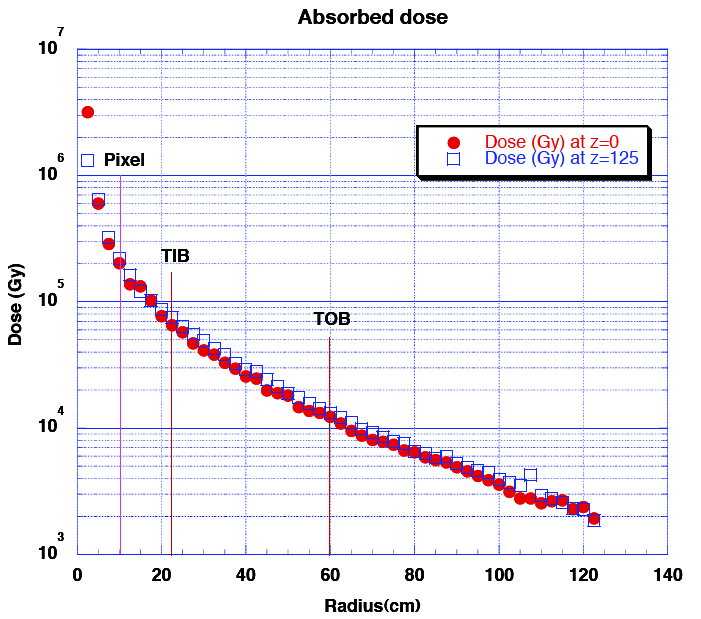
\includegraphics[width=0.8\textwidth]{021_pixel_upgrade/plots/irradiation_dose.png}
 \caption{The dose in Gy on to be absorbed by different tracker parts at different radial distance from the LHC $pp$ beam line for different
 $z$ coordinate values. The average position of the pixel detector is marked with a red vertical line. The location of different parts of the 
 silicon strip detector are also shown for comparison. The dose is defined for the expected full run time of the LHC until 2018, which 
 corresponds to the integrated luminosity of 500 fb$^{-1}$. The plot is taken from \cite{CMS:2012sda}.}
 \label{fig:irrad_dose}
\end{figure}

Here the studies of the properties of the irradiated prototype chips for layer 4 of BPIX will be presented. For this purpose the prototype
chips were irradiated at the CERN PS \cite{CERNTB} with the 23 GeV protons up to fluences of 3.8 $\cdot$ 10$^{14}$ $p/cm^{2}$ which corresponds to 
the expected lifetime dose of the layer 4 of the BPIX (approximately 16 MRad). 

The prototype chips were irradiated such that the silicon sensor side was facing the beam. The readout chips on the back side received a dose
up to 130 kGy. The tests  in the laboratory at DESY \cite{DESYWeb} showed the full functionality of the irradiated ROCs.

\subsection{DESY Beam Test}

To test the functionality of the prototype silicon pixel chip, one needs to deliver some particles with relatively high energy and let
the chip register them. For this purpose so called ``beam tests'' are performed. For the studies described in this thesis, the DESY beam test
facility was exploited.

The DESY beam test facility makes use of the electron-positron synchrotron DESY II \cite{Hemmie:1982xq, DESYIIWeb}, which provides electron
and positron beams with up to 1000 particles per cm$^{2}$ at energies of up to 6 GeV. However, these are not the particles which are directed
to the beam test areas. The circulating DESY II beam hits the 25$\mu$m thick carbon fiber and emits bremsstrahlung. The resulting photons are afterwards 
converted to electron-positron pairs on the converter, which is actually a copper plane. The resulting beam is passed to a dipole magnet for
separating the particles with the required momentum. Afterwards the beam is collimated and brought to the area where it can be exploited for the
experimental needs. The scheme of the facility which delivers the beam for the tests is shown in Fig. \ref{fig:desy_tb}.

\begin{figure}[t]
 \centering
 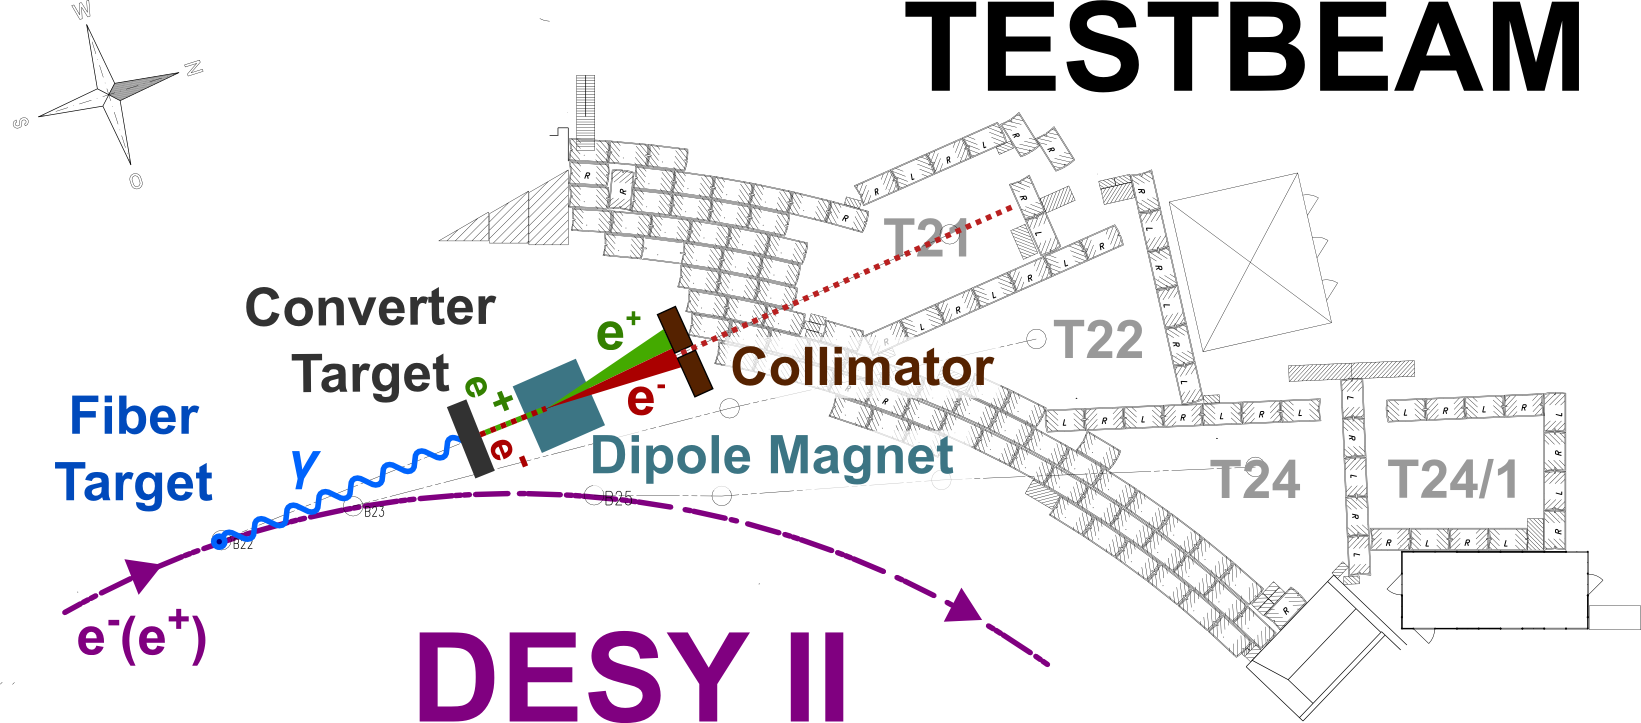
\includegraphics[width=1.0\textwidth]{021_pixel_upgrade/plots/desy_tb-sketch.png}
 \caption{Schematic layout of the test beam facility at DESY. The plot is taken from \cite{DESYTBArea}.}
 \label{fig:desy_tb}
\end{figure}

\subsection{EUDET Telescope and Experimental Setup} 

The beam test line where the tests described in this thesis were performed is equipped with a telescope of the EUDET/AIDA-family \cite{EUDET},
which is shown in Fig. \ref{fig:EUDET_tel}. It consists of two arms each equipped with three sensors kept at a stable temperature by a cooling
system. Each sensor plate can be moved along the beam axis to meet some particular experimental requirements.

\begin{figure}[t]
 \centering
 \includegraphics[width=1.0\textwidth]{021_pixel_upgrade/plots/Fig1.pdf}
 \caption{Photo of the EUDET telescope present at the beam test line 21 at DESY. The device under test is installed in between the two
 groups consisting of three telescope plates each. The electron/positron beam impinges perpendicularly onto the EUDET telescope planes 
 coming in from the right side of this photo.}
 \label{fig:EUDET_tel}
\end{figure}

The telescope serves as a device which measures the particle path with a very good precision so that it is assumed to be known.
The EUDET telescope is equipped with silicon pixels. The telescope sensors have a point precision of 3.4 $\mu$m and they
are made with a minimum of material (their thickness is only 50 $\mu$m), so that the precision doesn't drop even on the lowest 
energy border of the test beam ($\sim$ 1 GeV), when the contribution of the interaction of the particles with matter (multiple
scattering) becomes sizable. The installed Mimosa (Minimum Ionizing MOS Active Pixel Sensor) sensors (with a size of 
$21 \times 11$ mm$^{2}$ with squared pixels with s size of 18.4 $\mu$m) developed for the EUDET telescope make use of the MAPS 
(Monolitic Active Pixel Sensors) technology \cite{2001NIMPA.458..677T, Fischer:2002bv}.

The prototype silicon pixel chip for the BPIX upgrade was placed in between two arms of the telescope. In the beam test 
campaign the tested device (in case of these studies it's the prototype chip) is called a Device-Under-Test (DUT). The DUT
and it's board are placed in a special frame which allows tilting and turning (see Fig. \ref{fig:prototype_board}). 
This enables studies of the detector behavior with inclined particle tracks producing multi-pixel clusters. 

\begin{figure}[t]
 \centering
 \includegraphics[width=1.0\textwidth]{021_pixel_upgrade/plots/prototype_board.png}
 \caption{Photo of the DUT (prototype silicon pixel chip for the BPIX 4$^{th}$ layer upgrade) and it's board in the metal frame
 mounted between two arms of the EUDET telescope at the DESY beam test area.}
 \label{fig:prototype_board}
\end{figure}

There is a second CMS prototype chip placed downstream at the end of the beam telescope. It had to serve as a reference for the
measurement of the DUT efficiency, as it has the same time of the working cycle as the DUT (25 ns). The Mimosa has a much longer
cycle (115 $\mu$s) and it can't be used as a reference for the DUT.

On the front before and in right after the telescope two crossed scintillators are located. They serve as a trigger. 
If their signals coincide, the particle has passed all the way through the telescope.
The typical duration of one run when the telescope, DUT and reference chip were registering the test beam particles, was from 10
to 30 minutes having several hundred thousand trigger signals.

\subsection{Data Taking}

The data from the telescope was passed to the computer through network cables (see Fig. \ref{fig:EUDET_tel}) and from
the CMS prototype chips -- through USB cables (see Fig. \ref{fig:prototype_board}). These are the signals which inform
about the particles hitt the detector plane.  Afterwards the received data had to be preanalysed. 

To gain accurate knowledge of the geometry of the setup, alignment procedure was done with the Millipede algorithm 
\cite{1748-0221-3-09-P09002}.

The neighboring fired pixels on the pixel detector are grouped into clusters and the centers of the clusters are the hits.
The tracks were reconstructed from the hits using the general broken lines algorithm \cite{Blobel:2006yi}. It takes into
account the multiple scattering in the detector. 

To define the telescope resolution, first the particle track was reconstructed using the hits in the first and third telescope planes.
Then the second plane was used to determine the difference between the reconstructed particle track position and the actual hit in the 
second telescope plane.

This basic information from the telescope and from the prototype chips is used for the further analysis.

\subsection{Analyzing the Prototype Chip Properties}

Several crucial properties which are important for the future BPIX detector operation were measured during the DESY test beam 
campaign.

\subsubsection{Charge Collection}

The external bias voltage is needed to collect all the charge which was released due to the particle crossing the sensitive silicon
pixel of the detector. If the bias voltage is not high enough, not all the charge is collected and the particle energy may be defined
incorrectly. The voltage at which the full charge starts to be collected is called \textit{depletion voltage}. The bias voltage is
applied on the $p$-implant side. A schematic path of the ionizing particle through the silicon sensor and of the resulting charge 
collection is shown in \ref{fig:depl_volt}.

\begin{figure}[h]
 \centering
 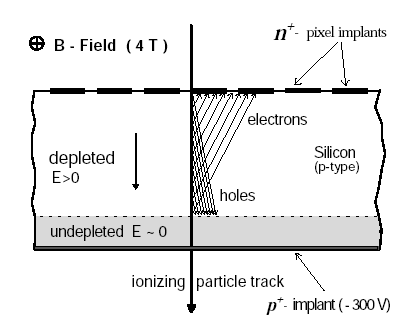
\includegraphics[width=0.6\textwidth]{021_pixel_upgrade/plots/depletion_voltage.png}
 \caption{The sketch of the charge collection from the ionizing particle crossing the silicon sensor. The figure is taken from \cite{}.}
 \label{fig:depl_volt}
\end{figure}

After the irradiation the damages in the silicon material are introduced. These damages may trap the ionized charge  which is traveling 
through the silicon to the place where it is read off. That is why a higher voltage is needed so that the particles overcome the traps.
However, there is a practical power dissipation related with the ohmic heating and on the bias voltage supply. If the depletion voltage
is higher than the voltage allowed by these limitations, the full depletion conditions for the sensors can never be reached. That is why 
it is necessary to test if the full depletion region can be reached and if so, then at which bias voltage.

To study this problem, the external bias voltage was varied from the very low values up to few hundred volts. The collected charge was
measured for each value of supplied bias voltage.

Fig. \ref{fig:depletion_voltage} shows the collected pixel cluster charge normalized to the maximum charge collected and tracking efficiency,
which was defined as the number of tracks which were registered in telescope, reference and DUT chips over the number
of tracks registered in telescope and reference chip.
These quantities are shown for two chips which were irradiated with doses of $0.9 \cdot 10^{14}$ p/cm$^2$ and $3.8 \cdot 10^{14}$ p/cm$^2$. 

\begin{figure}[t]
\centering
\begin{subfigure}
  \centering
  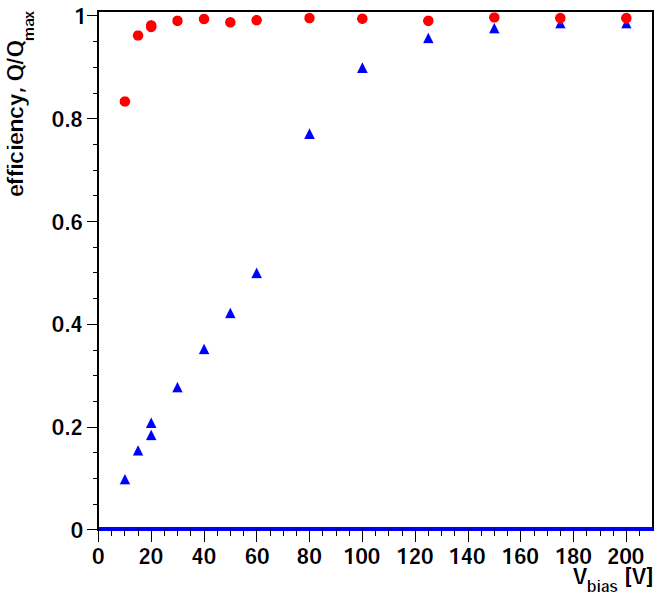
\includegraphics[width=0.42\textwidth]{021_pixel_upgrade/plots/voltage_scan_low_irrad.png}
\end{subfigure}
\begin{subfigure}
  \centering
  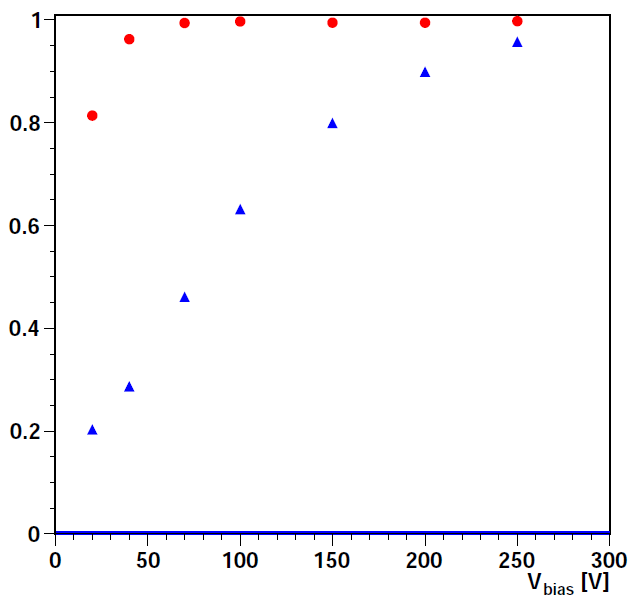
\includegraphics[width=0.4\textwidth]{021_pixel_upgrade/plots/voltage_scan_high_irrad.png}
\end{subfigure}
\caption{Charge collection efficiency, normalized to the maximum cluster charge (triangles) and tracking efficiency (circles) of the prototype silicon sensor
         for the CMS pixel tracker irradiated with $0.9 \cdot 10^{14}$ p/cm$^2$ (left) and $3.8 \cdot 10^{14}$ p/cm$^2$ (right) as function of the applied bias voltage.}
\label{fig:depletion_voltage}
\end{figure}

For the prototype chip which was irradiated with $0.9 \cdot 10^{14}$ p/cm$^2$, the collected charge drops quickly for bias voltages below -110 V. 
Only about one third of the charge is collected with a bias voltage lower than -30 V. However, the tracking efficiency still remains higher
than 90\%. This means, that the detector is fully efficient in terms of tracking with only one third of the charge collected.

For the chip with higher dose of $3.8 \cdot 10^{14}$ p/cm$^2$ full depletion is reached only with -250 V. The full tracking efficiency
is reached at -70 V, where around half of the charge was collected.

Additionally, the absolute pixel cluster charge distribution for the chip irradiated with a dose of $3.8 \cdot 10^{14}$ p/cm$^2$ was measured
with the -250 V bias voltage supplied (see Fig. \ref{fig:Landau}). It has an expected Landau shape, peaking at 18 ke. Before the irradiation a 
similar test was performed for this chip and Landau peak was at 22 ke then. This means that there is a charge loss due to trapping in the silicon
bulk after the irradiation.

\begin{figure}[t]
 \centering
 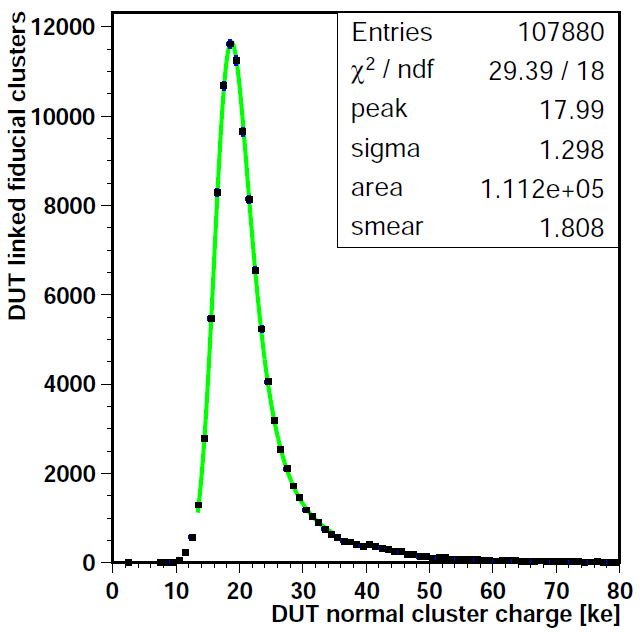
\includegraphics[width=0.6\textwidth]{021_pixel_upgrade/plots/Landau.png}
 \caption{Cluster charge distribution measured in the electron beam for a 285 $\mu$m thick pixel sensor irradiated with $3.8 \cdot 10^{14}$ p/cm$^2$ 
 at a bias voltage of -250 V (plateau region).}
 \label{fig:Landau}
\end{figure}

\subsubsection{Position Resolution}

The accuracy of the measurement of the position where the particle hit the silicon detector is primarily limited by the size of the silicon pixels.
However there is the way to improve the resolution using the charge sharing technique. If the charge from one particle will be collected in more
than one pixel, the position of the particle will be defined as the weighted average position of these pixels (the weighting is done corresponding 
to the amount of charge collected by each pixel). The charge sharing may happen either due to the inclined particle tracks with respect to the 
silicon sensor plane or because of the Lorentz drift in the magnetic field.

The particles from the DESY test beam were flying only in one direction. For the resolution improvement, the silicon chips were tilted by a certain 
angle with respect to the particle path to make the particles cross more than one pixel. This aims at obtaining an optimal charge sharing.

As discussed before, the irradiation introduces defects in the silicon which trap the charge carriers. This may influence the charge sharing
and thus the position resolution of the detector. It is also necessary to have the full charge collection to correctly measure the particle position.
Thus, the optimal bias voltage has to be delivered.

The resolution at the beam test was defined as the difference between the position of the particle hit defined by the DUT chip and the position of the
track defined in the telescope and extrapolated to the DUT. The telescope resolution (around 4.3 $\mu$m at 5 GeV beam energy and 150 mm spacing between
the telescope plane) is being quadratically subtracted.

To define the optimal tilt angle in the direction of the pixel rows of prototype chip, the DUT was tilted several times at different angles and the 
pixel row resolution\footnote{The \textit{row resolution} of the silicon pixel chip is the resolution of the coordinate in the pixel row direction. This
is the direction which an object would have if it would move from one row to the other staying inside one column.} was measured. Fig. \ref{fig:tilt_scan} 
shows the result of these studies for the prototype chip irradiated with a dose of $3.8 \cdot 10^{14}$ p/cm$^2$. As expected, first the resolution is 
getting better with increasing the tilt angle because the particle starts to pass through multiple pixels on it's way and the charge is shared between 
those pixels. After a certain optimal tilt angle, however, the resolution starts to get worse again. This is explained with a fact that the particle 
ionizes too many pixels initiating a very low charge in some of them. This charge doesn't overcome the threshold\footnote{A threshold on the charge 
collected is set on every pixel to avoid noise collection} level of a pixel and is lost. The plot shows that the minimum resolution is reached at 
the angle of around 20$^{o}$. Geometrically, the optimal charge sharing is expected at 19.3$^{o}$ tilt angle for 100 $\mu$m pixels and 285 $\mu$m 
sensor thickness. The higher angle which is practically measured may be explained by the trapping of deep charges. This means that the charges 
created in a silicon sensor by an ionizing particle trap on the defects starting from some depth of the sensor. Effectively it results in the
reduction of the sensitive thickness of the sensor, thus the tilt angle for an optimal charge sharing increases.

\begin{figure}[t]
 \centering
 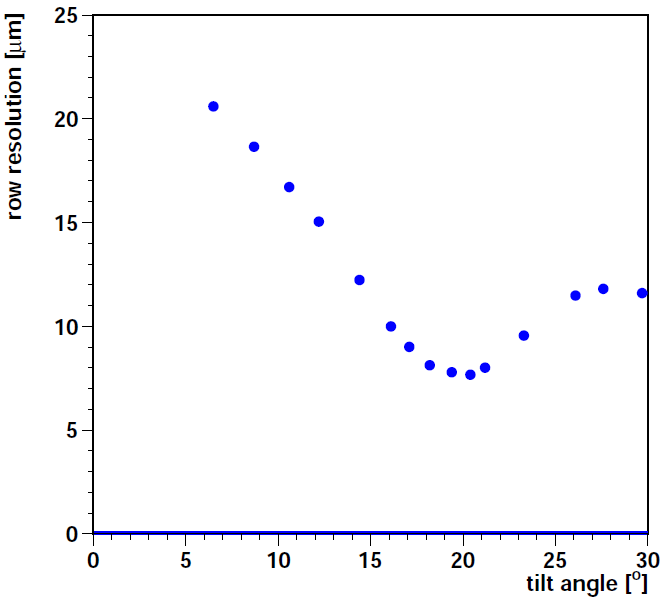
\includegraphics[width=0.55\textwidth]{021_pixel_upgrade/plots/tilt_scan.png}
 \caption{Resolution as a function of the tilt angle for a prototype silicon pixel module irradiated with $3.8 \cdot 10^{14}$ p/cm$^2$. The bias voltage  
 was set to -200 V and the threshold to 1.8 ke.}
 \label{fig:tilt_scan}
\end{figure}

For each point in Fig. \ref{fig:tilt_scan} the resolution in pixel row direction was determined as illustrated in Fig. \ref{fig:resol} using the 
width of the fitted gaussian. The plot shown is derived with the DUT tilted at 19$^{o}$.

\begin{figure}[t]
 \centering
 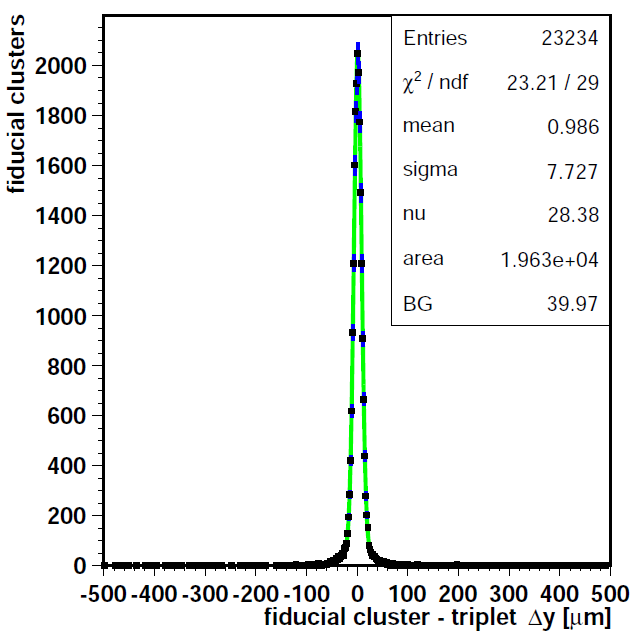
\includegraphics[width=0.6\textwidth]{021_pixel_upgrade/plots/resol_dist.png}
 \caption{Residual between DUT cluster position and telescope track in the direction of the 100 $\mu$m pixel size at a bias voltage of -320 V. The sensor 
 was tilted by an angle of 19$^{o}$ to the beam direction. The charge threshold was set to 1.8 ke. The fluence is $3.8 \cdot 10^{14}$ p/cm$^2$.}
 \label{fig:resol}
\end{figure}

The position resolution in the row direction was also measured for different bias voltages supplied. The result is presented in Fig. \ref{fig:bias_res}.
It shows that reducing the bias voltage below 150 V leads to a resolution degradation.

\begin{figure}[t]
 \centering
 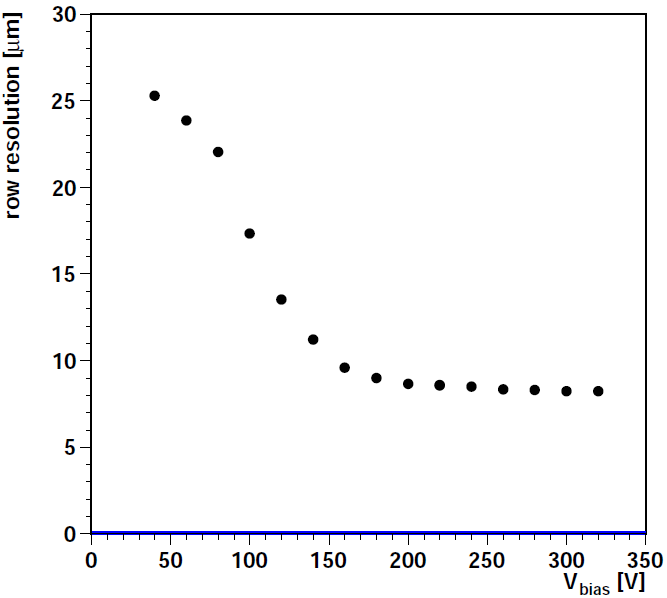
\includegraphics[width=0.55\textwidth]{021_pixel_upgrade/plots/bias_resol.png}
 \caption{Resolution as a function of the applied bias voltage without subtracting the telescope contribution, for a prototype silicon pixel module 
 irradiated with $3.8 \cdot 10^{14}$ p/cm$^2$.}
 \label{fig:bias_res}
\end{figure}

\subsection{Summary}

The prototype chips for the layer 4 of silicon pixel tracker for the CMS Phase 1 upgrade were operating after absorbing doses in order of and 
much higher than expected to be absorbed during the detector operation time. The damage effects caused by irradiation are observed. However,
the chips are fully operable and produce reasonable results. The resolution only slightly degrades -- the irradiated prototype has the resolution
of 6.4 $\mu$m in row direction, while before the irradiation this value was 5.5 $\mu$m. The full depletion after is reached at 150 V after the
irradiation.

In summary the tests of the prototype chips indicate that these types of chips meet the demands for operation after Phase I upgrade.